
\chapter{Continuation}
\label{chap:cont_appendix}

\section{Harmonic balance}
\label{sec:hb_appendix}

Figure \ref{fig:hb_frf_appendix} shows the influence of the included number of
harmonics $N_H$, The time discretisation $N$ and the optimal number of
iterations $I_{opt}$. Fig. \ref{fig:hb_frf_a_appendix} shows superharmonic
resonances at low frequencies are not captured for $N_H=3$ and $N_H=1$. This is
expected as they possesses multiple frequency content, but shows that care
should be taken when the number of harmonics is selected. Especially for more
complicated and rich vibrations that this simple example.
For systems with few DOFs, it is not a problem to include a high number of
harmonics - remember that system matrices $\bm A$ in the HB method, eq
\eqref{eq:hb_A}, is of size $(2N_H + 1)n \times (2N_H + 1)n$ and the sparse
Fourier operator $\bm \Gamma$ of size $nH \times(2N_H+1)n$ where $n$ is number
of DOFs. But for large systems it will become a problem. To solve this,
\citet{GROLET2012a} present a way to automatically adopt the number of harmonics
for each DOF.

Fig. \ref{fig:hb_frf_b_appendix} shows that the solution is inaccurate around
the peak for lower $N$. This is due to aliasing effects.{\textbf -- Det slap du
  nu lidt for nemt om ved --}

Fig. \ref{fig:hb_frf_c_appendix} shows that the peak is ``cut short'' or
truncated for higher values of $I_{opt}$. Setting a high value of $I_{opt}$
allows for taking larger steps, since more Newton iterations are allowed to
correct the guess. Thus resolution is decreased. Of course one can use a
\texttt{max\_step} parameter to prevent too large steps.

\begin{figure}[ht!]
  \centering
  \begin{subfigure}[b]{0.7\textwidth}
    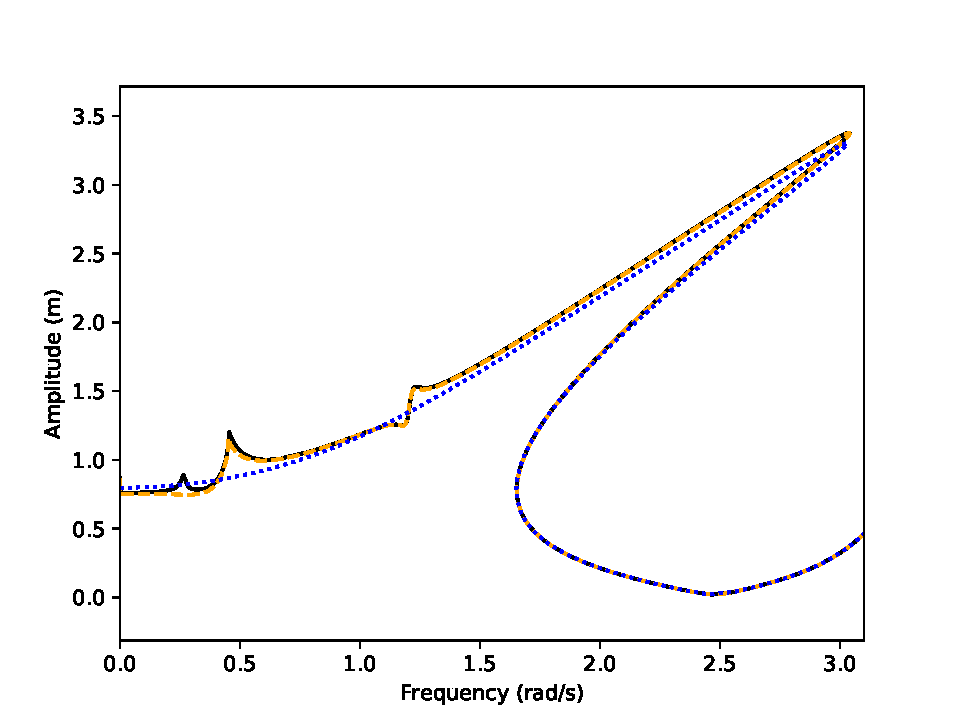
\includegraphics[width=\linewidth, height=8cm]{2dof_duffing/hb_nh.tikz}
    \caption{}
    \label{fig:hb_frf_a_appendix}
  \end{subfigure}\\
  \begin{subfigure}[b]{0.45\textwidth}
    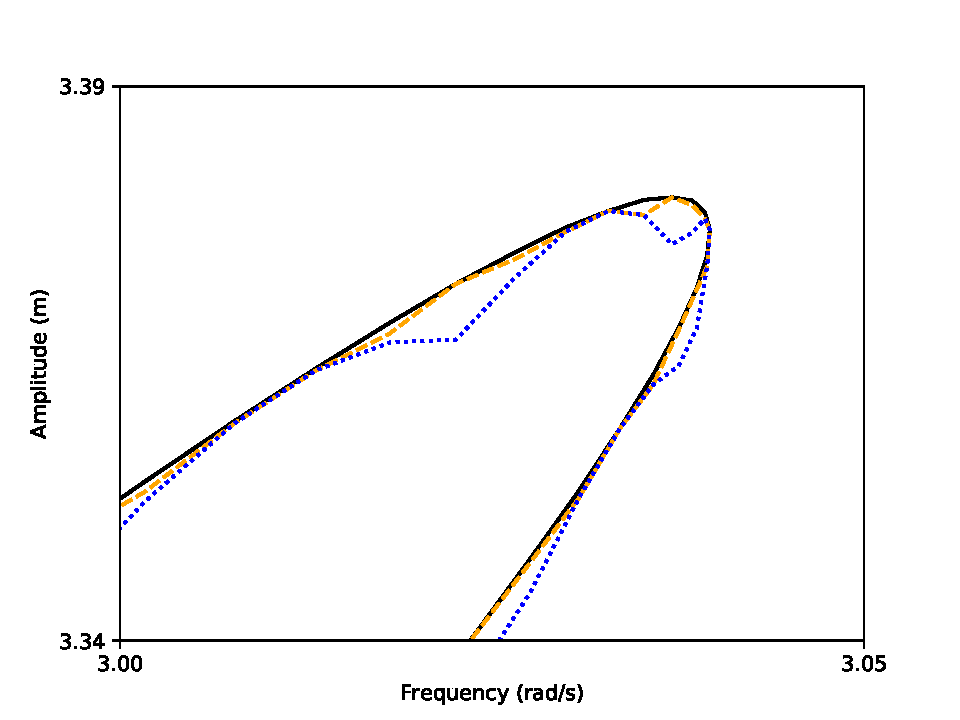
\includegraphics[width=\linewidth, height=5cm]{2dof_duffing/hb_N.tikz}
    \caption{}
    \label{fig:hb_frf_b_appendix}
  \end{subfigure}~
  \begin{subfigure}[b]{0.45\textwidth}
    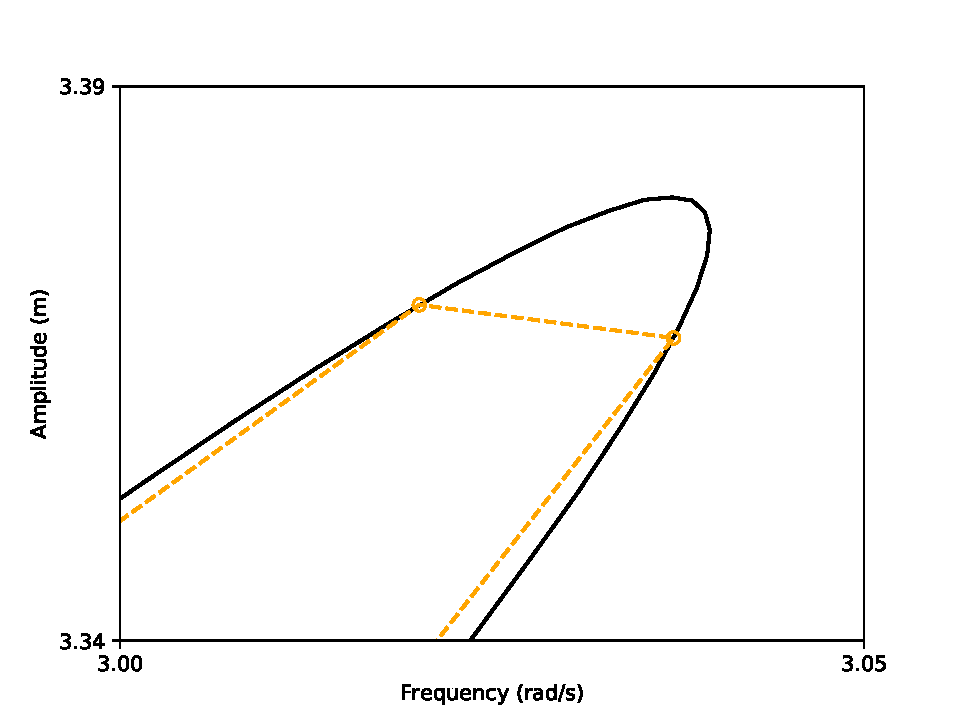
\includegraphics[width=\linewidth, height=5cm]{2dof_duffing/hb_ipopt.tikz}
    \caption{}
    \label{fig:hb_frf_c_appendix}
  \end{subfigure}
  \caption{NRFC of the coupled duffing system for $x_1$ with $f=2$N. Influence
    of HB and continuation parameters, compared to $N_H=5, N=512, I_{opt}=3$ (\sampleline{}).
    Stability is not shown.
    \textbf{(a)}
    (\sampleline{dashed}) $N_H=3$;
    (\sampleline{dotted}) $N_H=1$;
    \textbf{(b)}
    (\sampleline{dashed}) $N=128$;
    (\sampleline{dotted}) $N=64$;
    \textbf{(c)}
    (\sampleline{dashed}) $I_{opt}=5$;}
  \label{fig:hb_frf_appendix}
\end{figure}




%%% Local Variables:
%%% mode: latex
%%% TeX-master: "../../report"
%%% End:
